\documentclass[aspectratio=1610,12pt,notheorems]{beamer}

\usepackage[utf8x]{inputenc} \usepackage[russian]{babel}
\usepackage{amsmath,amssymb,amsthm,mathtools}
\usepackage{graphicx,caption,subcaption}
\usepackage{hyperref,natbib}
\usepackage{tikz,xcolor,colortbl,makecell}
\usepackage{algorithm,algpseudocode}
\usepackage{qrcode}

\usetikzlibrary{arrows,backgrounds,patterns,%
	matrix,shapes,fit,calc,shadows,plotmarks,snakes}

\theoremstyle{plain}
\newtheorem{theorem}{Теорема}
\newtheorem{lemma}[theorem]{Лемма}

\theoremstyle{definition}
\newtheorem{definition}{Определение}
\newtheorem{problem}{Задача}

\usetheme[height=0.97cm]{Rochester}
\usecolortheme{dolphin}

\definecolor{hard}{RGB}{145,55,55}
\definecolor{mnsgold}{RGB}{240,235,220}

\setbeamercolor{headline}{bg=hard,fg=mnsgold}
\setbeamercolor*{frametitle}{parent=headline}

\setbeamercolor{structure}{fg=hard}
\setbeamercolor{subsection in head/foot}{bg=white,fg=hard}
\setbeamercolor{section in head/foot}{bg=hard,fg=mnsgold}
\setbeamercolor{block title}{bg=hard,fg=mnsgold}

\setbeamertemplate{navigation symbols}{}

\parskip=2.6mm
\def\ll{\left(} \def\rr{\right)}
\def\lag{\left\langle} \def\rag{\right\rangle}

\definecolor{failpos}{RGB}{230,30,20}
\definecolor{initpos}{RGB}{30,20,220}
\definecolor{turna}{RGB}{100,240,110}
\definecolor{turnb}{RGB}{250,140,110}

\newcommand{\vseper}{\vphantom{$\int_{0_0}^{0^0}$}}

\newcommand{\singlepayoff}[2]{\tikz{
	\draw (0,0) node{\vseper #1}; \draw (0.8,0.8) node{\vseper #2};
}}

\newcommand{\rowdescription}[1]{\tikz{
	\draw (0,0) node{\vseper #1}; \draw (0,0.8) node{\vseper};
}}

\newcommand{\coldescription}[1]{\tikz{
	\draw (0,0) node{\vseper}; \draw (0.8,0) node{\vseper #1};
}}

\newcommand{\myref}[2]{\href{#1}{\texttt{\underline{#2}}}}

\def\mitem{\medskip\item}
\def\ps{\\ [0.65cm]} \linespread{1.16}
\def\fram#1#2{\begin{frame}\frametitle{#1}#2\end{frame}}
\def\usl#1#2{\begin{block}{#1} #2 \end{block} \medskip\pause}
\def\uslnp#1#2{\begin{block}{#1} #2 \end{block} \medskip}
\def\mov#1#2{\begin{scope}[xshift = #1 cm] #2 \end{scope};}

\def\divsby{\mathrel{\rlap{.}\rlap{\raisebox{0.55ex}{.}}\raisebox{1.1ex}{.}}}
\definecolor{starvert}{RGB}{110,175,230}
\newcommand{\vfi}{\varphi}
\newcommand{\litem}{\vspace{0.5cm}\item}

\newcommand{\nkstar}[2]{
	\foreach \i in {1,...,#1} {\draw[thick] (90 + 360 * \i / #1 : 3.5)
		-- (90 + 360 * \i / #1 + 360 * #2 / #1 : 3.5);}
	\foreach \i in {1,...,#1} {\fill[starvert] (90 + 360 * \i / #1 : 3.5) circle[radius=0.16cm];}
}

\title[Solutions of MNS]
    {\bfseries Решения избранных задач}

\author[\ ]
	{Б. А. Золотов,\quad «Математика НОН-СТОП»\\ \vspace{0.3cm}
		{\small Фонд «Время Науки»}}

\institute[\ ]{\ }

\date{4 декабря 2020}

%%%%%%%%%%%%%%
%%%%%%%%%%%%%%

\begin{document}

\frame{\titlepage}


%%%%%% 4 класс, кубики
\begin{frame} \frametitle{Кубики}
\begin{figure}[h] \centering
    \tikz[scale=0.47]{
    {
    \draw[black!50!white,thick]{ (-4,2)--(4,2)--(4,4)--(-4,4)--(-4,2)
    (-2,2)--(-2,6)--(0,6)--(0,0)--(2,0)--(2,4)
    }
    }
    %6
    {
    {\fill[black] (-1.4,5.5) circle (0.15cm)}
    {\fill[black] (-0.6,5.5) circle (0.15cm)}
    {\fill[black] (-1.4,5) circle (0.15cm)}
    {\fill[black] (-0.6,5) circle (0.15cm)}
    {\fill[black] (-1.4,4.5) circle (0.15cm)}
    {\fill[black] (-0.6,4.5) circle (0.15cm)}
    }
    %5
    {
    {\fill[black] (-3,3) circle (0.15cm)}
    {\fill[black] (-3.4,3.4) circle (0.15cm)}
    {\fill[black] (-3.4,2.6) circle (0.15cm)}
    {\fill[black] (-2.6,3.4) circle (0.15cm)}
    {\fill[black] (-2.6,2.6) circle (0.15cm)}
    }
    %4
    {
    {\fill[black] (-1.4,3.4) circle (0.15cm)}
    {\fill[black] (-1.4,2.6) circle (0.15cm)}
    {\fill[black] (-0.6,3.4) circle (0.15cm)}
    {\fill[black] (-0.6,2.6) circle (0.15cm)}
    }
    %2
    {
    {\fill[black] (1.4,3.4) circle (0.15cm)}
    {\fill[black] (0.6,2.6) circle (0.15cm)}
    }
    %3
    {
    {\fill[black] (3.4,3.4) circle (0.15cm)}
    {\fill[black] (3,3) circle (0.15cm)}
    {\fill[black] (2.6,2.6) circle (0.15cm)}
    }
    %1
    {
    {\fill[black] (1,1) circle (0.15cm)} } }
\end{figure}


	\usl{2020-4-6B}{Сколько видимых точек может быть на башне из $6$ кубиков?}

Сумма чисел на противоположных гранях равна 7. \medskip \pause

Ответ — $84 + k$.
\end{frame}


%%%%%% 4 класс, разрезания
\begin{frame} \frametitle{Кирпичей}

\usl{2020-4-4C}{
	Нарисуйте на клетчатой бумаге такую фигуру, которую
	можно разделить по клеткам на 2, на 3, на 4, на 5, на 6
	одинаковых по форме и размеру связных фигур~—
	причём они не будут прямоугольниками.
}

\begin{center} \tikz[scale=0.28]
{
   \foreach \x / \y in {
	1/1, 1/2, 1/3, 1/4, 1/5, 1/6, 1/7, 1/8, 1/9, 1/10,  %делим на 2
	2/2, 2/3, 2/4, 2/5, 2/6, 2/7, 2/8, 2/9, 2/10, 2/11,
	3/1, 3/2, 3/3, 3/4, 3/5, 3/6, 3/7, 3/8, 3/9, 3/10,
	9/1, 9/2, 9/3, 9/4, 9/5, 9/6, 9/7, 9/8, 9/9, 9/10,  %делим на 3
	10/2, 10/3, 10/4, 10/5, 10/6, 10/7, 10/8, 10/9, 10/10, 10/11,
	13/1, 13/2, 13/3, 13/4, 13/5, 13/6, 13/7, 13/8, 13/9, 13/10,
	14/2, 14/3, 14/4, 14/5, 14/6, 14/7, 14/8, 14/9, 14/10, 14/11,
	17/1, 17/2, 17/3, 17/4, 17/5,    %делим на 4
	18/2, 18/3, 18/4, 18/5, 18/6,
	19/1, 19/2, 19/3, 19/4, 19/5, 
	20/7, 20/8, 20/9, 20/10, 20/11,
	21/6, 21/7, 21/8, 21/9, 21/10,
	22/7, 22/8, 22/9, 22/10, 22/11,
	25/3, 25/4, 25/7, 25/8,     %делим на 5
	26/4, 26/5, 26/8, 26/9, 
	27/3, 27/4, 27/7, 27/8, 
	28/4, 28/5, 28/8, 28/9, 
	29/3, 29/4, 29/7, 29/8, 
	30/4, 30/5, 30/8, 30/9, 
	33/1, 33/2, 33/3, 33/4, 33/5,     %делим на 6
	34/2, 34/3, 34/4, 34/5, 34/6, 
	35/6, 35/7, 35/8, 35/9, 35/10,
	36/7, 36/8, 36/9, 36/10, 36/11,
	37/1, 37/2, 37/3, 37/4, 37/5, 
	38/2, 38/3, 38/4, 38/5, 38/6, 38/7
   } 
   \draw[fill opacity=0.6] (\x, \y) rectangle (\x cm + 1 cm, \y cm + 1 cm);
   \foreach \x / \y in {
	4/2, 4/3, 4/4, 4/5, 4/6, 4/7, 4/8, 4/9, 4/10, 4/11,    %делим на 2
	5/1, 5/2, 5/3, 5/4, 5/5, 5/6, 5/7, 5/8, 5/9, 5/10,
	6/2, 6/3, 6/4, 6/5, 6/6, 6/7, 6/8, 6/9, 6/10, 6/11,
	11/1, 11/2, 11/3, 11/4, 11/5, 11/6, 11/7, 11/8, 11/9, 11/10,    %делим на 3
	12/2, 12/3, 12/4, 12/5, 12/6, 12/7, 12/8, 12/9, 12/10, 12/11,
	17/6, 17/7, 17/8, 17/9, 17/10,    %делим на 4
	18/7, 18/8, 18/9, 18/10, 18/11,
	19/6, 19/7, 19/8, 19/9, 19/10,
	20/2, 20/3, 20/4, 20/5, 20/6, 
	21/1, 21/2, 21/3, 21/4, 21/5, 
	22/2, 22/3, 22/4, 22/5, 22/6,
	25/1, 25/2, 25/5, 25/6, 25/9, 25/10,     %делим на 5
	26/2, 26/3, 26/6, 26/7, 26/10, 26/11,
	27/1, 27/2, 27/5, 27/6, 27/9, 27/10,
	28/2, 28/3, 28/6, 28/7, 28/10, 28/11,
	29/1, 29/2, 29/5, 29/6, 29/9, 29/10,
	30/2, 30/3, 30/6, 30/7, 30/10, 30/11,
	33/6, 33/7, 33/8, 33/9, 33/10,     %делим на 6
	34/7, 34/8, 34/9, 34/10, 34/11,
	35/1, 35/2, 35/3, 35/4, 35/5,
	36/2, 36/3, 36/4, 36/5, 36/6,
	37/6, 37/7, 37/8, 37/9, 37/10,
	38/8, 38/9, 38/10, 38/11
   } 
   \draw[fill=gray,fill opacity=0.6] (\x, \y) rectangle (\x cm + 1 cm, \y cm + 1 cm);
   \node at (2.5,6.5) {1};     %нумеруем 2
   \node at (5.5,6.5) {2};
   \node at (9.5,6.5) {1};     %нумеруем 3
   \node at (11.5,6.5) {2};
   \node at (13.5,6.5) {3};
   \node at (18.5,9.5) {1};     %нумеруем 4
   \node at (21.5,8.5) {2};
   \node at (18.5,4.5) {3};
   \node at (21.5,3.5) {4};
   \node at (27.5,9.5) {1};     %нумеруем 5
   \node at (27.5,7.5) {2};
   \node at (27.5,5.5) {3};
   \node at (27.5,3.5) {4};
   \node at (27.5,1.5) {5};
   \node at (33.5,9.5) {1};     %нумеруем 6
   \node at (35.5,9.5) {2};
   \node at (37.5,9.5) {3};
   \node at (33.5,4.5) {4};
   \node at (35.5,4.5) {5};
   \node at (37.5,4.5) {6};
} 
\end{center}
\end{frame}


%%%%%% 5 класс, разрезания
\begin{frame} \frametitle{Разрезания}
	\usl{2020-5-1C}{
		Можно ли нарисовать на клетчатом листе бумаги такую фигуру, которую можно разрезать по линиям сетки на две {\itshape одинаковые} фигуры двумя способами~— причём фигуры в первом и во втором способе были бы одни и те же, но линии разреза выглядели бы по-разному?
	}

\begin{center} \tikz[scale=0.75]
{
   \foreach \x / \y in {
	1/3, 2/3, 3/3, 3/4, 6/1, 6/2, 6/3, 7/3
   } 
	\draw[thick,fill opacity=0.6] (\x, \y) rectangle (\x cm + 1 cm, \y cm + 1 cm);
   {
   \foreach \x / \y in {
	1/1, 1/2, 2/2, 3/2, 7/2, 8/2, 8/3, 8/4
   } 
	\draw[thick,fill=gray,fill opacity=0.6] (\x, \y) rectangle (\x cm + 1 cm, \y cm + 1 cm);
	\node at (1.5,2.5) {$A$};
	\node at (3.5,3.5) {$B$};
	\node at (6.5,3.5) {$B$};
	\node at (8.5,2.5) {$A$};
}
} 
\end{center}
\end{frame}


%%%%%% 5 класс, семнашка, 4 пары
\begin{frame} \frametitle{Семнадцатый независимый}

\usl{2020-5-3A}{
	Песню каждого участника оценивает 15 судей. Судья ставит каждому участнику в паре от 0 до 22 баллов и отдаёт свой голос участнику, которому поставил больше баллов. В паре объявляется победителем тот участник, которому отдано больше голосов. Может ли быть так, что победитель в паре набрал меньше баллов, чем проигравший, несмотря на перевес в голосах?
}

\end{frame}

\begin{frame} \frametitle{Семнадцатый независимый}

\newcommand{\vs}{&\hspace{-3mm}:&\hspace{-3mm}}
\begin{center} \begin{tabular}{|l|rcl|rcl|c|c|}
	\hline
	Участник & \multicolumn{3}{c|}{Победы}
		& \multicolumn{3}{c|}{Проигрыши}
		& Баллы & Голоса \\ \hline \hline
	Победитель 1 & 1 \vs 0 & 0 \vs 22 & 11 & 11 \\ \hline
	Победитель 2 & 2 \vs 0 & 0 \vs 16 & 20 & 10 \\ \hline
	Победитель 3 & 3 \vs 0 & 0 \vs 12 & 27 & 9 \\ \hline
	Победитель 4 & 4 \vs 0 & 0 \vs 9 & 32 & 8 \\ \hline \hline
	Проигравший 4 & 9 \vs 0 & 0 \vs 4 & 63 & 7 \\ \hline
	Проигравший 3 & 12 \vs 0 & 0 \vs 3 & 72 & 6 \\ \hline
	Проигравший 2 & 16 \vs 0 & 0 \vs 2 & 80 & 5 \\ \hline
	Проигравший 1 & 22 \vs 0 & 0 \vs 1 & 88 & 4 \\ \hline
\end{tabular} \end{center}

\end{frame}


%%%%%% 6 класс, научки
\begin{frame} \frametitle{Опубликовать за 60 секунд}
	\usl{2020-6-2B}{
	Научные руководители придумывают темы работ.
     \begin{itemize}
	\item Один из них придумывает 1 новую тему;
	\item После этого кто-то из них придумывает 2 новых темы;
	\item После этого кто-то из них придумывает 3 новых темы.
     \end{itemize}
	Пусть изначально первый придумал на $n$ тем больше, чем второй. Докажите, что руководители всегда смогут сравнять количество придуманных ими тем.
	}

Каждые два хода разность количеств тем будем сокращать на 1.
\end{frame}


%%%%%% 6 класс, сортировка
\begin{frame} \frametitle{Сортировка}
Выпишем все числа от одного до десяти — но не в привычном порядке возрастания, а в алфавитном порядке: восемь, два, девять, десять, один, пять, семь, три, четыре, шесть. \medskip

\usl{2020-6-4B}{
Числа от 1 до 10'000'000'000 (десять миллиардов) выписали в алфавитном порядке. Перечислите первые десять из них.
}

(1) 18 (2) 18 миллионов (3) 18 миллионов 18 (4) 18 миллионов 18 тысяч \\
(5) 18 миллионов 18 тысяч 18 (6) \ldots восемь (7) \ldots восемьдесят \\
(8) \ldots 88 (9) \ldots 82 (10) \ldots 89.
\end{frame}


%%%%%% 6 класс, пульт от кондиционера
\begin{frame} \frametitle{Пульт от кондиционера}
\begin{center} 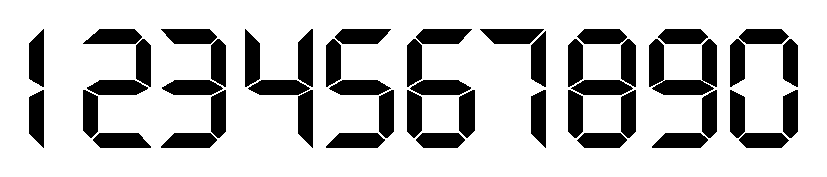
\includegraphics[width=6.8cm]{img/Digiface} \end{center}

	\usl{2020-6-5A}{На пульте есть две кнопки: «предыдущий режим» и «следующий режим». Работают только сегменты, образующие цифру 7. Сколько переключений тогда нужно, чтобы гарантированно определить режим, в котором находится пульт?}

\begin{center} 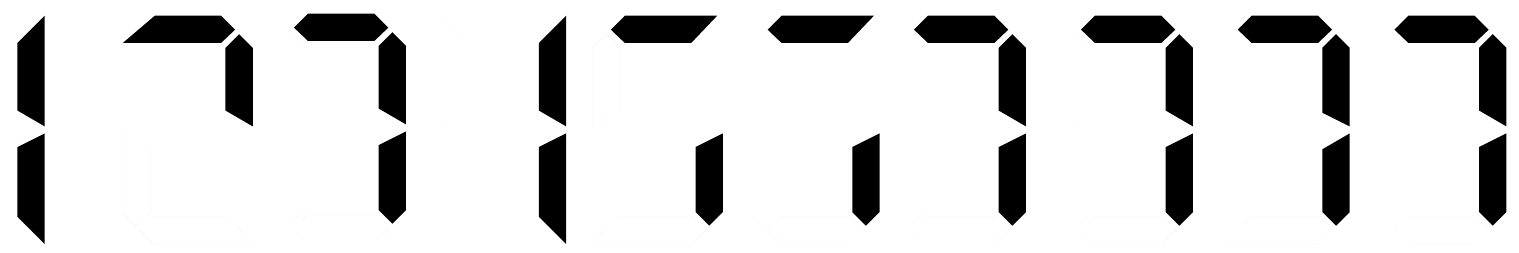
\includegraphics[width=6.3cm]{img/Digiface-A} \end{center}
\end{frame}


%%%%%% 7 класс, делимость в системе счисления
\begin{frame} \frametitle{Системы счисления и делимость}

\usl{2020-7-8C}{Число $N$ записывается в системе счисления с основанием $n$ как\\
		\centerline{$(n-1)(n-1)(n-1)(n-1)0$.}
Докажите, что число $N$ делится на три последовательных натуральных числа.}

Делится на $n-1$, $n$, $n+1$ (оно записывается как 11). \medskip \pause

А также на 1, 2, 3: $n(n-1)(n^3+n^2+n+1) = n(n-1)(n+1)(n^2+1)$.


\end{frame}


%%%%%% 8 класс, факториалы
\begin{frame} \frametitle{Факториалы и простые множители}

Рассмотрим множество $M$ степеней двойки, в которых она может входить в разложение факториала на простые множители.

Число $4$ лежит в множестве $M$\!, потому что $6! = 2^4 \cdot 3^2 \cdot 5$. \medskip

\usl{2020-8-7B}{Докажите, что если числа $a$ и $a+1$ принадлежат $M$\!, то $a+2$ не принадлежит $M$\!.}

$t_1$ — наибольшее, $t_1! = 2^a \cdot r$.

$t_2$ — наименьшее, $t_2! = 2^{a+1} \cdot r$. Тогда $t_2$ не делится на 4, а следующее чётное число делится на 4.

\end{frame}


%%%%%% Профиль
\begin{frame} \frametitle{Профильные задания}
{\it Система високосных лет} для числа $t$ — это последовательность натуральных чисел $(a_0, a_2, a_3, \ldots, a_n)$ такая, что $a_{i+1}$ делится на $a_i$, а также
	$$\frac{1}{a_0} - \frac{1}{a_1} + \frac{1}{a_2} - \frac{1}{a_3} + \ldots
	     + (-1)^{n} \cdot \frac{1}{a_n}\ =\ t.$$ \smallskip

Какой могла бы быть система високосных лет, если бы длина года составляла 365.21875, 365.17, 365.33 дней? Для любого ли рационального числа существует система високосных лет?
\end{frame}

\begin{frame} \frametitle{Профильные задания}

\begin{align*}
	& 365.21875 = 365 + \frac{1}{4} - \frac{1}{32}
		\vphantom{\int\limits_{0_0}^{0^0}} \\
	& 365.17 = 365 + \frac{1}{5} - \frac{1}{25} + \frac{1}{100}
		\vphantom{\int\limits_{0_0}^{0^0}} \\
	& 365.33 = 365 + \frac{1}{3} - \frac{1}{300}
		\vphantom{\int\limits_{0_0}^{0^0}} \\
\end{align*}

\end{frame}

\begin{frame} \begin{center}
\ 

	{\Large Спасибо за внимание!} \vspace{0.4cm}

	{\large \url{mathnonstop.ru}}

	{\large \url{mathnonstop@timeforscience.ru}}

	{\large \url{vk.com/timeforscience}}
\end{center} \end{frame}

\end{document}
